\documentclass[12pt,a4paper]{article}

% Margins.
\setlength{\oddsidemargin}{0in}
\setlength{\evensidemargin}{0in}
\setlength{\headheight}{12pt}
\setlength{\headsep}{42pt}
\setlength{\topmargin}{-54pt}
\setlength{\textwidth}{6.5in}
\setlength{\textheight}{9in}

\usepackage{amsmath}
\usepackage{float}
\usepackage{graphicx}
% Drawing.
\usepackage{pgf}
\usepackage{tikz}

% Listings for formatting code.
\usepackage{listings}
% General options.
\lstset{breaklines=true, basicstyle=\small\ttfamily, tabsize=4, numbers=left, stepnumber=1, frame=single, showstringspaces=false}
% C++ specific high-lighting. Comments are 50/50 shades of green/black and strings coloured with 60/40 red/black mixture.
\lstset{language=[ISO]C++, commentstyle=\color{green!50!black}, keywordstyle=\color{blue}, stringstyle=\color{red!60!black}}

%opening
\title{\vspace{-2cm}Programming for Engineers I\\Lab 12\\Pointers and Arrays}
\author{Hina Ashraf\and Attique Dawood}

\begin{document}
\maketitle
\section{Pointers}
A pointer is a variable that stores address of another variable. This pointer essentially `points' to that variable. Pointer can be used to change the value of variable it points.
\begin{lstlisting}[caption={Pointers}]
#include <cstdio>
int main()
{
	int a=3; // A simple int.
	int* ap; // A pointer of type int.
	ap = &a; // Pointer ap now points to int a.
	*ap = 5; // Changes value of a to 5 from 3.

	printf("%d\n", a);  // Print value of a.
	printf("%d\n", &a); // Print address of a.
	printf("%d\n", ap); // Print value of ap, which is address of a.
	printf("%d\n", *a); // Print value of a using pointer ap.

	return 0;
}
\end{lstlisting}
\section{Using Pointers for Referencing}
Since pointers point to original variables they can be used to change the value of original variables in a function call.
\begin{lstlisting}[caption={Pointers as Arguments}]
#include <cstdio>
int Area(int*, int*); // Function prototype.
int main()
{
	int a, b, c;
	a = 3;
	b = 5;
	c = Area(&a, &b); // Function call by address.
	
	return 0;
}
// Function definition.
int Area(int* x, int* y)
{
	int z = (*x)*(*y); // Dereferencing pointers.
	*x=7; // Changes value of a in main().
	return z;
}
\end{lstlisting}
\section{Pointers and Arrays}
The name of array is the pointer to its first element. A subscript besides array name can be translated in english as, ``access element located this much distance from start.'' Keep in mind that \verb|Array[i]| is the same as \verb|*(Array+i)| which means that you only need array pointer to access array elements using the subscript. Consider the following code
\begin{lstlisting}[caption={Arrays and Pointers}]
#include <cstdio>
int Area(int*, int*); // Function prototype.
int main()
{
	int Array[5] = {3,7,2,1,5};

	printf("%d\n", Array); // Prints the address of array.

	// Using subscript.
	printf("%d\n", Array[0]); // Print the value of element located a distance of 0 from start.
	printf("%d\n", Array[3]); // Print the value of element located a distance of 3 from start.
	printf("%d\n", Array[5]); // Print the value of element located a distance of 5 from start. ERROR! Out of bound.

	// Using Pointers.
	printf("%d\n", *(Array+0)); // Prints the value of first element which is 3.
	printf("%d\n", *(Array+1)); // Prints the value of second element which is 7.
	printf("%d\n", *(Array+5)); // Prints the value of sixth element which out of bound or ERROR.

	return 0;
}
\end{lstlisting}
\begin{figure}[H]
\centering
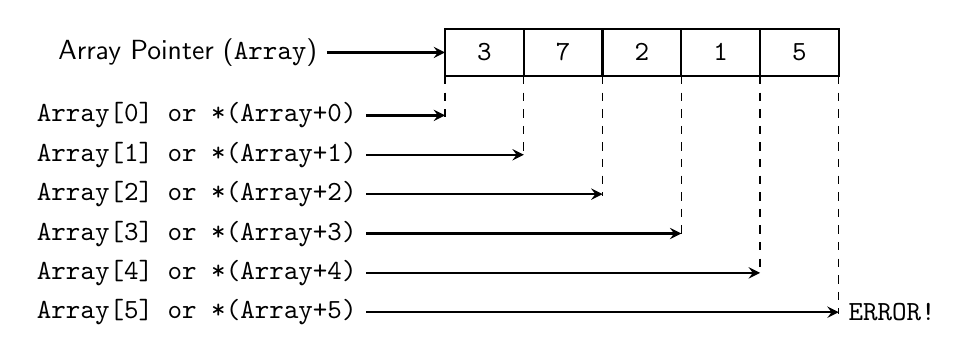
\begin{tikzpicture}
	% Writing 'Array'
	\coordinate [label=left:\textsf{Array Pointer (\texttt{Array})}] (Arraypointer) at (-1.5cm,0.3cm);
	\draw[thick, ->, >=stealth] (-1.5cm, 0.3cm) -- (0cm, 0.3cm);
	% Drawing boxes.
	\foreach \x in {0.0cm, 1.0cm, 2.0cm, 3.0cm, 4.0cm}
		\draw[thick] (\x, 0cm) rectangle (\x+1.0cm, 0.6cm);
	% Writing numbers in boxes. This is original array.
	\foreach \x/\y in {0.0cm/3, 1.0cm/7, 2.0cm/2, 3.0cm/1, 4.0cm/5}
		\draw (\x+0.5cm,0.3cm) node {\texttt{\y}};
	\def\XD{0cm}
	\def\YD{-0.5cm}
	% Drawing an arrow and pointer.
	\coordinate [label=left:\texttt{Array[0] or *(Array+0)}] (Array0) at (-1cm,\YD);
	\draw[thick, ->, >=stealth] (-1cm, \YD) -- (0cm+\XD, \YD);
	\draw[dashed] (\XD,0cm) -- (\XD,\YD-0.5);

	\def\XD{1cm}
	\def\YD{-1cm}
	% Drawing an arrow and pointer.
	\coordinate [label=left:\texttt{Array[1] or *(Array+1)}] (Array1) at (-1cm,\YD);
	\draw[thick, ->, >=stealth] (-1cm, \YD) -- (0cm+\XD, \YD);
	\draw[dashed] (\XD,0cm) -- (\XD,\YD-0.5);

	\def\XD{2cm}
	\def\YD{-1.5cm}
	% Drawing an arrow and pointer.
	\coordinate [label=left:\texttt{Array[2] or *(Array+2)}] (Array2) at (-1cm,\YD);
	\draw[thick, ->, >=stealth] (-1cm, \YD) -- (0cm+\XD, \YD);
	\draw[dashed] (\XD,0cm) -- (\XD,\YD-0.5);

	\def\XD{3cm}
	\def\YD{-2cm}
	% Drawing an arrow and pointer.
	\coordinate [label=left:\texttt{Array[3] or *(Array+3)}] (Array3) at (-1cm,\YD);
	\draw[thick, ->, >=stealth] (-1cm, \YD) -- (0cm+\XD, \YD);
	\draw[dashed] (\XD,0cm) -- (\XD,\YD-0.5);
	
	\def\XD{4cm}
	\def\YD{-2.5cm}
	% Drawing an arrow and pointer.
	\coordinate [label=left:\texttt{Array[4] or *(Array+4)}] (Array4) at (-1cm,\YD);
	\draw[thick, ->, >=stealth] (-1cm, \YD) -- (0cm+\XD, \YD);
	\draw[dashed] (\XD,0cm) -- (\XD,\YD-0.5);
	
	\def\XD{5cm}
	\def\YD{-3cm}
	% Drawing an arrow and pointer.
	\coordinate [label=left:\texttt{Array[5] or *(Array+5)}] (Array5) at (-1cm,\YD);
	\draw[thick, ->, >=stealth] (-1cm, \YD) -- (0cm+\XD, \YD);
	\draw[dashed] (\XD,0cm) -- (\XD,\YD-0.5);
	\coordinate [label=right:\texttt{ERROR!}] (Error) at (\XD,\YD);
\end{tikzpicture}
\caption{Using pointer to access array elements}
\label{Array-pointer-element-access}
\end{figure}
\section{Exercise}
\textbf{Question No. 1:} Write a C Program to find maximum and minimum element in an array. There must be a function that receives an array of 10 integers as one of the arguments. In this function, find minimum and maximum integer from the array passed to it. Send the result (minimum and maximum value/element) back to main(). No global variables should be used. Declare the array of 10 integers in the main() and take the values as input from the user. Call the above mentioned function from main() and print the results (maximum and minimum values) in main(). You must not calculate minimum and maximum values in main(); instead only print the results (sent back by the function) in main(). You are supposed to do these using pointers. Do all array indexes access using pointer notation.\\
\\
\textbf{Question No. 2:} Write a simple program to calculate the first 100 primes, and store them in increasing order in an array. (Note: Use pointer notation in your program and perform the above task using functions)\\
Remember the definition of a prime number:
A prime number is any integer strictly greater than 1, which can only be divided by itself and 1.\\
\\
\textbf{Question No. 3:} Write a program to compute $e^x$. $n$ and $x$ should be input by user. The number of terms to compute will be $n+1$. It would be convenient to write a function that calculates factorial of a number. Also, keep in mind $0! = 1$, same as $1! = 1$.
\begin{equation}
e^x = 1+\dfrac{x^1}{1!}+\dfrac{x^2}{2!}+\dfrac{x^3}{3!}+\dfrac{x^4}{4!}+\dfrac{x^5}{5!}+\dfrac{x^6}{6!}+...+\dfrac{x^n}{n!}.
\label{eq:ex-Taylor-Series}
\end{equation}
\begin{figure}[H]
\centering
\begin{tikzpicture}
	\newcommand{\Xdisp}{0cm}
	\newcommand{\Ydisp}{0cm}
	% e^x;
	\coordinate [label=center:$e^x\rightarrow$] (exequals) at (\Xdisp-0.75cm,\Ydisp+0.75cm);
	% Single-threaded flow chart.
	\draw (\Xdisp-0.25cm,\Ydisp+0.75cm) -- (\Xdisp+0.5cm,\Ydisp+0.75cm) -- (\Xdisp+0.5cm,\Ydisp);
	\draw (\Xdisp,\Ydisp) rectangle (\Xdisp+1.0cm,\Ydisp-1.0cm);
	\coordinate [label=center:$\dfrac{x^0}{0!}$] (Term0ST) at (\Xdisp+0.5cm,\Ydisp-0.5cm);

	\renewcommand{\Xdisp}{1.25cm}
	\renewcommand{\Ydisp}{-1.25cm}
	\draw (\Xdisp-0.25cm,\Ydisp+0.75cm) -- (\Xdisp+0.5cm,\Ydisp+0.75cm) -- (\Xdisp+0.5cm,\Ydisp);
	\draw (\Xdisp,\Ydisp) rectangle (\Xdisp+1.0cm,\Ydisp-1.0cm);
	\coordinate [label=center:$\dfrac{x^1}{1!}$] (Term1ST) at (\Xdisp+0.5cm,\Ydisp-0.5cm);
	\filldraw[fill=white] (\Xdisp+0.5cm,\Ydisp+0.75cm) circle (0.25cm);
	\coordinate [label=center:$+$] (plusTerm1ST) at (\Xdisp+0.5cm,\Ydisp+0.75cm);

	\renewcommand{\Xdisp}{2.5cm}
	\renewcommand{\Ydisp}{-2.5cm}
	\draw (\Xdisp-0.25cm,\Ydisp+0.75cm) -- (\Xdisp+0.5cm,\Ydisp+0.75cm) -- (\Xdisp+0.5cm,\Ydisp);
	\draw (\Xdisp,\Ydisp) rectangle (\Xdisp+1.0cm,\Ydisp-1.0cm);
	\coordinate [label=center:$\dfrac{x^2}{2!}$] (Term2ST) at (\Xdisp+0.5cm,\Ydisp-0.5cm);
	\filldraw[fill=white] (\Xdisp+0.5cm,\Ydisp+0.75cm) circle (0.25cm);
	\coordinate [label=center:$+$] (plusTerm2ST) at (\Xdisp+0.5cm,\Ydisp+0.75cm);

	\renewcommand{\Xdisp}{3.75cm}
	\renewcommand{\Ydisp}{-3.75cm}
	\draw (\Xdisp-0.25cm,\Ydisp+0.75cm) -- (\Xdisp+0.5cm,\Ydisp+0.75cm) -- (\Xdisp+0.5cm,\Ydisp);
	\draw (\Xdisp,\Ydisp) rectangle (\Xdisp+1.0cm,\Ydisp-1.0cm);
	\coordinate [label=center:$\dfrac{x^3}{3!}$] (Term3ST) at (\Xdisp+0.5cm,\Ydisp-0.5cm);
	\filldraw[fill=white] (\Xdisp+0.5cm,\Ydisp+0.75cm) circle (0.25cm);
	\coordinate [label=center:$+$] (plusTerm3ST) at (\Xdisp+0.5cm,\Ydisp+0.75cm);

	\renewcommand{\Xdisp}{5cm}
	\renewcommand{\Ydisp}{-5cm}
	\draw[dashed] (\Xdisp-0.25cm,\Ydisp+0.75cm) -- (\Xdisp+0.5cm,\Ydisp+0.75cm) -- (\Xdisp+0.5cm,\Ydisp);
	\draw (\Xdisp,\Ydisp) rectangle (\Xdisp+1.0cm,\Ydisp-1.0cm);
	\coordinate [label=center:$\dfrac{x^n}{n!}$] (TermnST) at (\Xdisp+0.5cm,\Ydisp-0.5cm);
	\filldraw[fill=white] (\Xdisp+0.5cm,\Ydisp+0.75cm) circle (0.25cm);
	\coordinate [label=center:$+$] (plusTermnST) at (\Xdisp+0.5cm,\Ydisp+0.75cm);
	% Result
	\coordinate [label=right:$\rightarrow$\textsf{Result}] (ResultST) at (\Xdisp+1.0cm,\Ydisp-0.5cm);
	% Thread.
	\draw[thick, rounded corners, ->, >=stealth] (-0.75cm,-0.5cm) -- (-0.9cm,-0.75cm) -- (-0.6cm,-1.25cm) -- (-0.9cm,-1.75cm) -- (-0.6cm,-2.25cm) -- (-0.9cm,-2.75cm) -- (-0.6cm,-3.25cm) -- (-0.9cm,-3.75cm) -- (-0.6cm,-4.25cm) -- (-0.9cm,-4.75cm) -- (-0.75cm,-5.0cm) -- (-0.75cm,-5.5cm);
\end{tikzpicture}
\caption{Series computation of $e^x$}
\label{fig:Series-computation-ex}
\end{figure}
\end{document}
